\documentclass{article}

\usepackage[a4paper,margin=2cm]{geometry}
\usepackage{array}
\usepackage{amsmath}
\usepackage{amsfonts}
\usepackage{fancyhdr}
\usepackage{tabularx}

\usepackage{tikz}
\usepackage{pgfplots}

\usepackage{enumitem}

\usepackage{float}

\usepackage{caption}

\lhead{Name:}

\chead{Trigonometrie}

\rhead{Datum: \hphantom{dd.MM.yyyy}}

\pagestyle{fancy}

\pgfplotsset{compat=1.18}

\begin{document}

\section*{Trigonometrie}

\subsection*{Polarform}

\begin{enumerate}[label=$\bullet$]
    \item Ein Koordinatensystem
    \item Für Komplexe Zahlen gedacht 
    \item Hat einen Pol O, Polarachse, Winkel $\theta$ und länge $r$
    \item Die Polarkoordinatendarstellung ist $P(r, \theta)$
    \item $r \in \mathbb{R}+$ und $\theta \in [0, 2\pi)$
\end{enumerate}

\fbox{$r = \sqrt{x^2 + y^2}$}

\fbox{$\theta = atan2(y,x)$}

$\operatorname{atan2}(y,x) = \begin{cases}
    \arctan\left(\frac{y}{x}\right) & \text{if } x > 0 \\
    \arctan\left(\frac{y}{x}\right) + \pi & \text{if } x < 0 \text{ and } y \geq 0 \\
    \arctan\left(\frac{y}{x}\right) - \pi & \text{if } x < 0 \text{ and } y < 0 \\
    +\frac{\pi}{2} & \text{if } x = 0 \text{ and } y > 0 \\
    -\frac{\pi}{2} & \text{if } x = 0 \text{ and } y < 0 \\
    \text{undefined} & \text{if } x = 0 \text{ and } y = 0
\end{cases}$

\subsection*{Sinus, Cosinus, Tangens}

%plot sin, cos, tan
\begin{figure}[H]
    \centering
    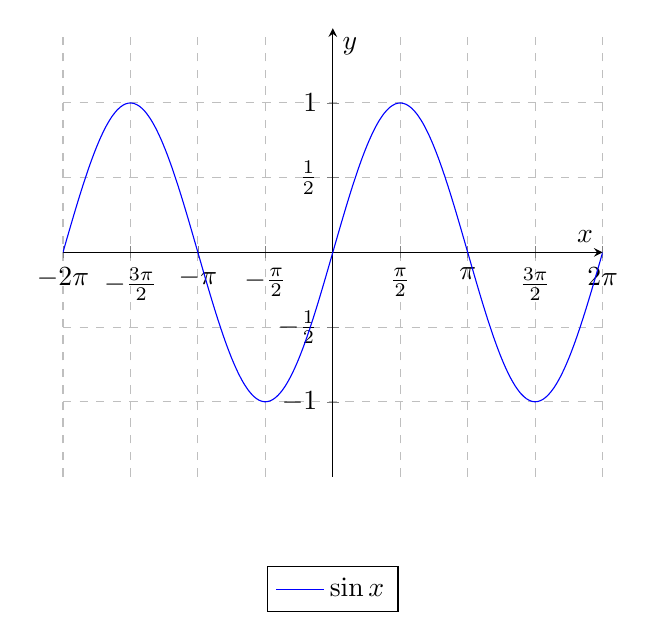
\begin{tikzpicture}
        \begin{axis}[
            xlabel=$x$,
            ylabel=$y   $,
            xmin=-2*pi,
            xmax=2*pi,
            ymin=-1.5,  
            ymax=1.5,
            xtick={-2*pi,-3*pi/2,-pi,-pi/2,0,pi/2,pi,3*pi/2,2*pi},
            xticklabels={$-2\pi$,$-\frac{3\pi}{2}$,$-\pi$,$-\frac{\pi}{2}$,$0$,$\frac{\pi}{2}$,$\pi$,$\frac{3\pi}{2}$,$2\pi$},
            ytick={-1,-0.5,0,0.5,1},
            yticklabels={$-1$,$-\frac{1}{2}$,$0$,$\frac{1}{2}$,$1$},
            grid=major,
            grid style=dashed,
            legend pos=north west,
            legend cell align=left,
            legend columns=3,
            legend style={at={(0.5,-0.2)},anchor=north},
            axis lines=middle,
            ]
            \addplot[domain=-2*pi:2*pi,samples=100,smooth,blue] {sin(deg(x))};
            \legend{$\sin x$}
        \end{axis}
    \end{tikzpicture}
    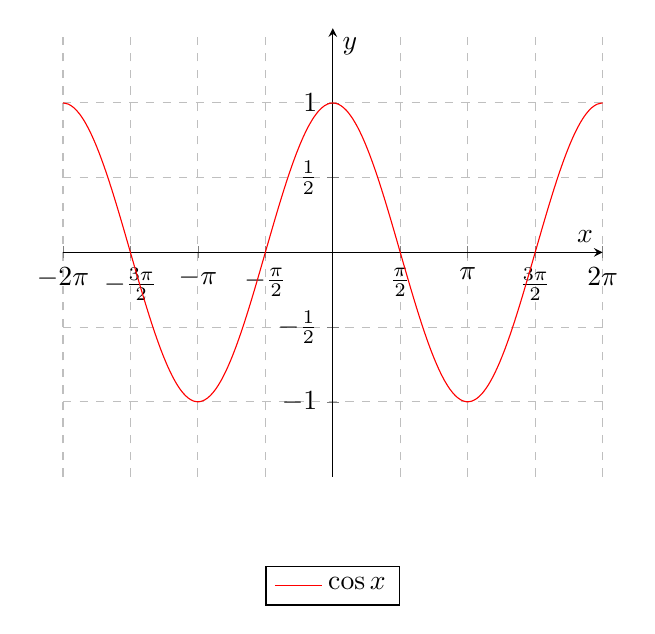
\begin{tikzpicture}
        \begin{axis}[
            xlabel=$x$,
            ylabel=$y   $,
            xmin=-2*pi,
            xmax=2*pi,
            ymin=-1.5,  
            ymax=1.5,
            xtick={-2*pi,-3*pi/2,-pi,-pi/2,0,pi/2,pi,3*pi/2,2*pi},
            xticklabels={$-2\pi$,$-\frac{3\pi}{2}$,$-\pi$,$-\frac{\pi}{2}$,$0$,$\frac{\pi}{2}$,$\pi$,$\frac{3\pi}{2}$,$2\pi$},
            ytick={-1,-0.5,0,0.5,1},
            yticklabels={$-1$,$-\frac{1}{2}$,$0$,$\frac{1}{2}$,$1$},
            grid=major,
            grid style=dashed,
            legend pos=north west,
            legend cell align=left,
            legend columns=3,
            legend style={at={(0.5,-0.2)},anchor=north},
            axis lines=middle,
            ]
            \addplot[domain=-2*pi:2*pi,samples=100,smooth,red] {cos(deg(x))};
            \legend{$\cos x$}
        \end{axis}
    \end{tikzpicture}
    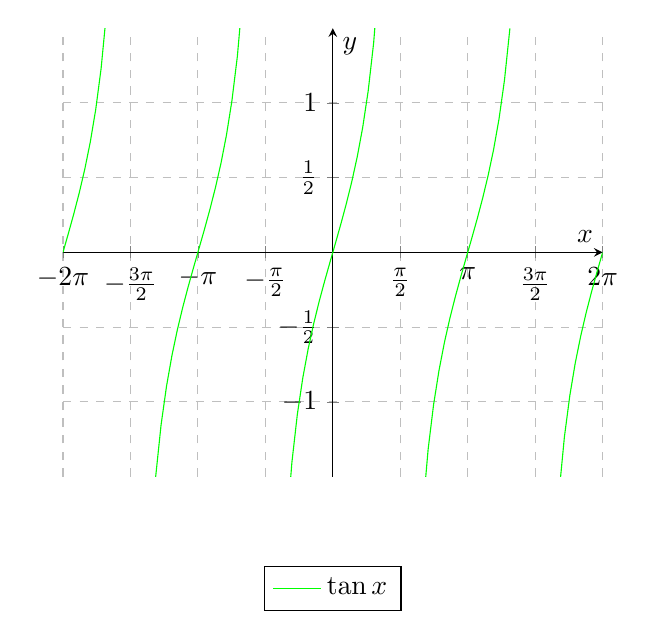
\begin{tikzpicture}
        \begin{axis}[
            xlabel=$x$,
            ylabel=$y   $,
            xmin=-2*pi,
            xmax=2*pi,
            ymin=-1.5,  
            ymax=1.5,
            xtick={-2*pi,-3*pi/2,-pi,-pi/2,0,pi/2,pi,3*pi/2,2*pi},
            xticklabels={$-2\pi$,$-\frac{3\pi}{2}$,$-\pi$,$-\frac{\pi}{2}$,$0$,$\frac{\pi}{2}$,$\pi$,$\frac{3\pi}{2}$,$2\pi$},
            ytick={-1,-0.5,0,0.5,1},
            yticklabels={$-1$,$-\frac{1}{2}$,$0$,$\frac{1}{2}$,$1$},
            grid=major,
            grid style=dashed,
            legend pos=north west,
            legend cell align=left,
            legend columns=3,
            legend style={at={(0.5,-0.2)},anchor=north},
            axis lines=middle,
            domain=-2*pi:2*pi,
            restrict y to domain=-2:2,
            ]
            \addplot[samples=100, green] {tan(deg(x))};
            \legend{$\tan x$}
        \end{axis}
    \end{tikzpicture}
    \captionsetup{labelformat=empty}
\end{figure}


\subsection*{Trigonometrischer Pythagoras}

\begin{figure}[H]
    \centering
    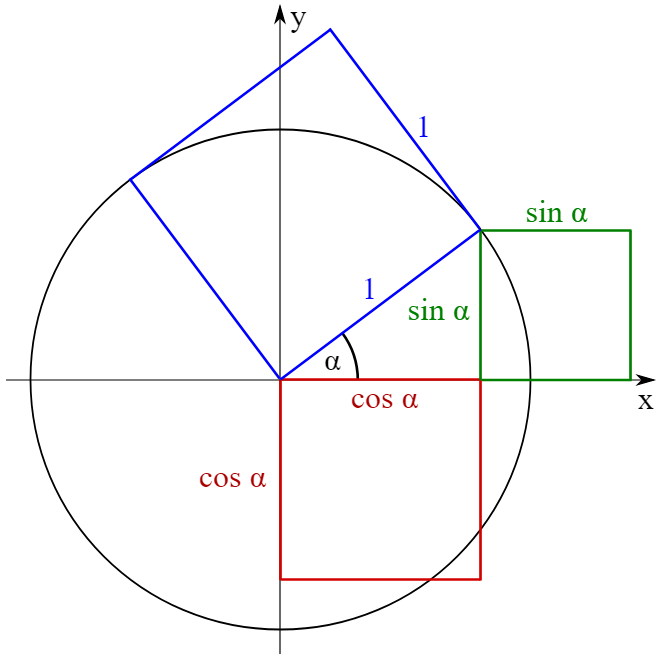
\includegraphics[width=0.25\linewidth]{image2.png}
    \captionsetup{labelformat=empty}
\end{figure}

\fbox{$\sin^2\theta + \cos^2\theta = 1$}

\subsection*{Additionstheoreme}

\begin{figure}[H]
    \centering
    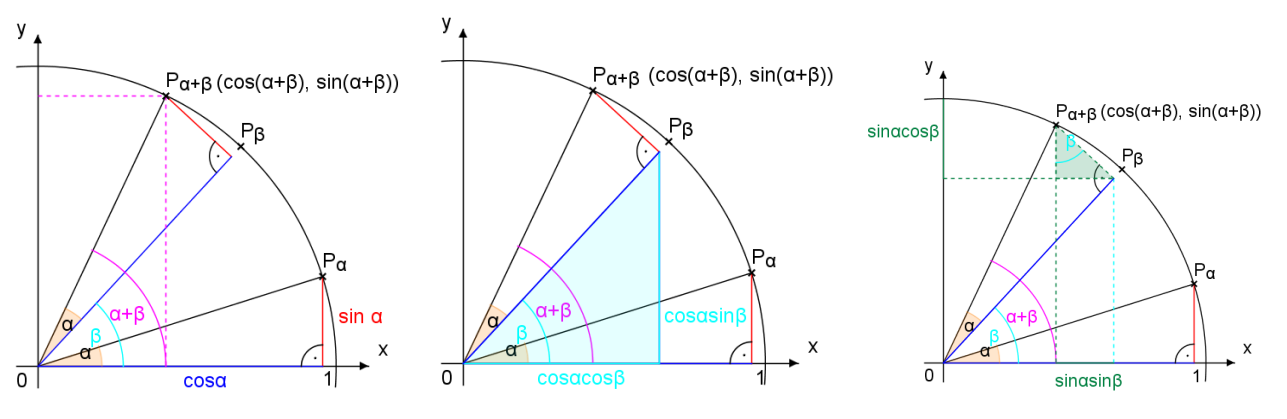
\includegraphics[width=0.85\linewidth]{image3.png}
    \captionsetup{labelformat=empty}
\end{figure}

\begin{enumerate}[label=$\bullet$]
    \item $\sin{(\alpha + \beta)} = \sin\alpha \cos\beta + \cos\alpha \sin\beta$
    \item $\cos{(\alpha + \beta)} = \cos\alpha \cos\beta - \sin\alpha \sin\beta$
\end{enumerate}

\subsection*{Eigenschaften}

\begin{enumerate}[label=$\bullet$]
    \item $\sin{(\pi - \theta)} =  \sin\theta$
    \item $\cos{(\pi - \theta)} = -\cos\theta$
    \item $\tan{(\pi - \theta)} = -\tan\theta$ \\
    
    \item $\sin{(\theta + k \cdot 2\pi)} = \sin\theta \hspace*{15pt} \theta \in [0, 2\pi]$
    \item $\cos{(\theta + k \cdot 2\pi)} = \cos\theta \hspace*{15pt} \theta \in [0, 2\pi]$
    \item $\tan{(\theta + k \cdot 2\pi)} = \tan\theta \hspace*{15pt} \theta \in [0, 2\pi]$ \\
    
    \item $\sin{(- \theta)} = -\sin\theta \mid \mbox{Punktsymmetrie}$
    \item $\cos{(- \theta)} =  \cos\theta \mid \mbox{Achsensymmetrie}$
    \item $\tan{(- \theta)} = -\tan\theta \mid \mbox{Punktsymmetrie}$ \\
    
    \item $\sin\theta = \cos(\theta - \frac{\pi}{2})$
    \item $\cos\theta = \sin(\theta + \frac{\pi}{2})$
\end{enumerate}

\subsection*{Ableitungen}

\begin{figure}[H]
    \centering
    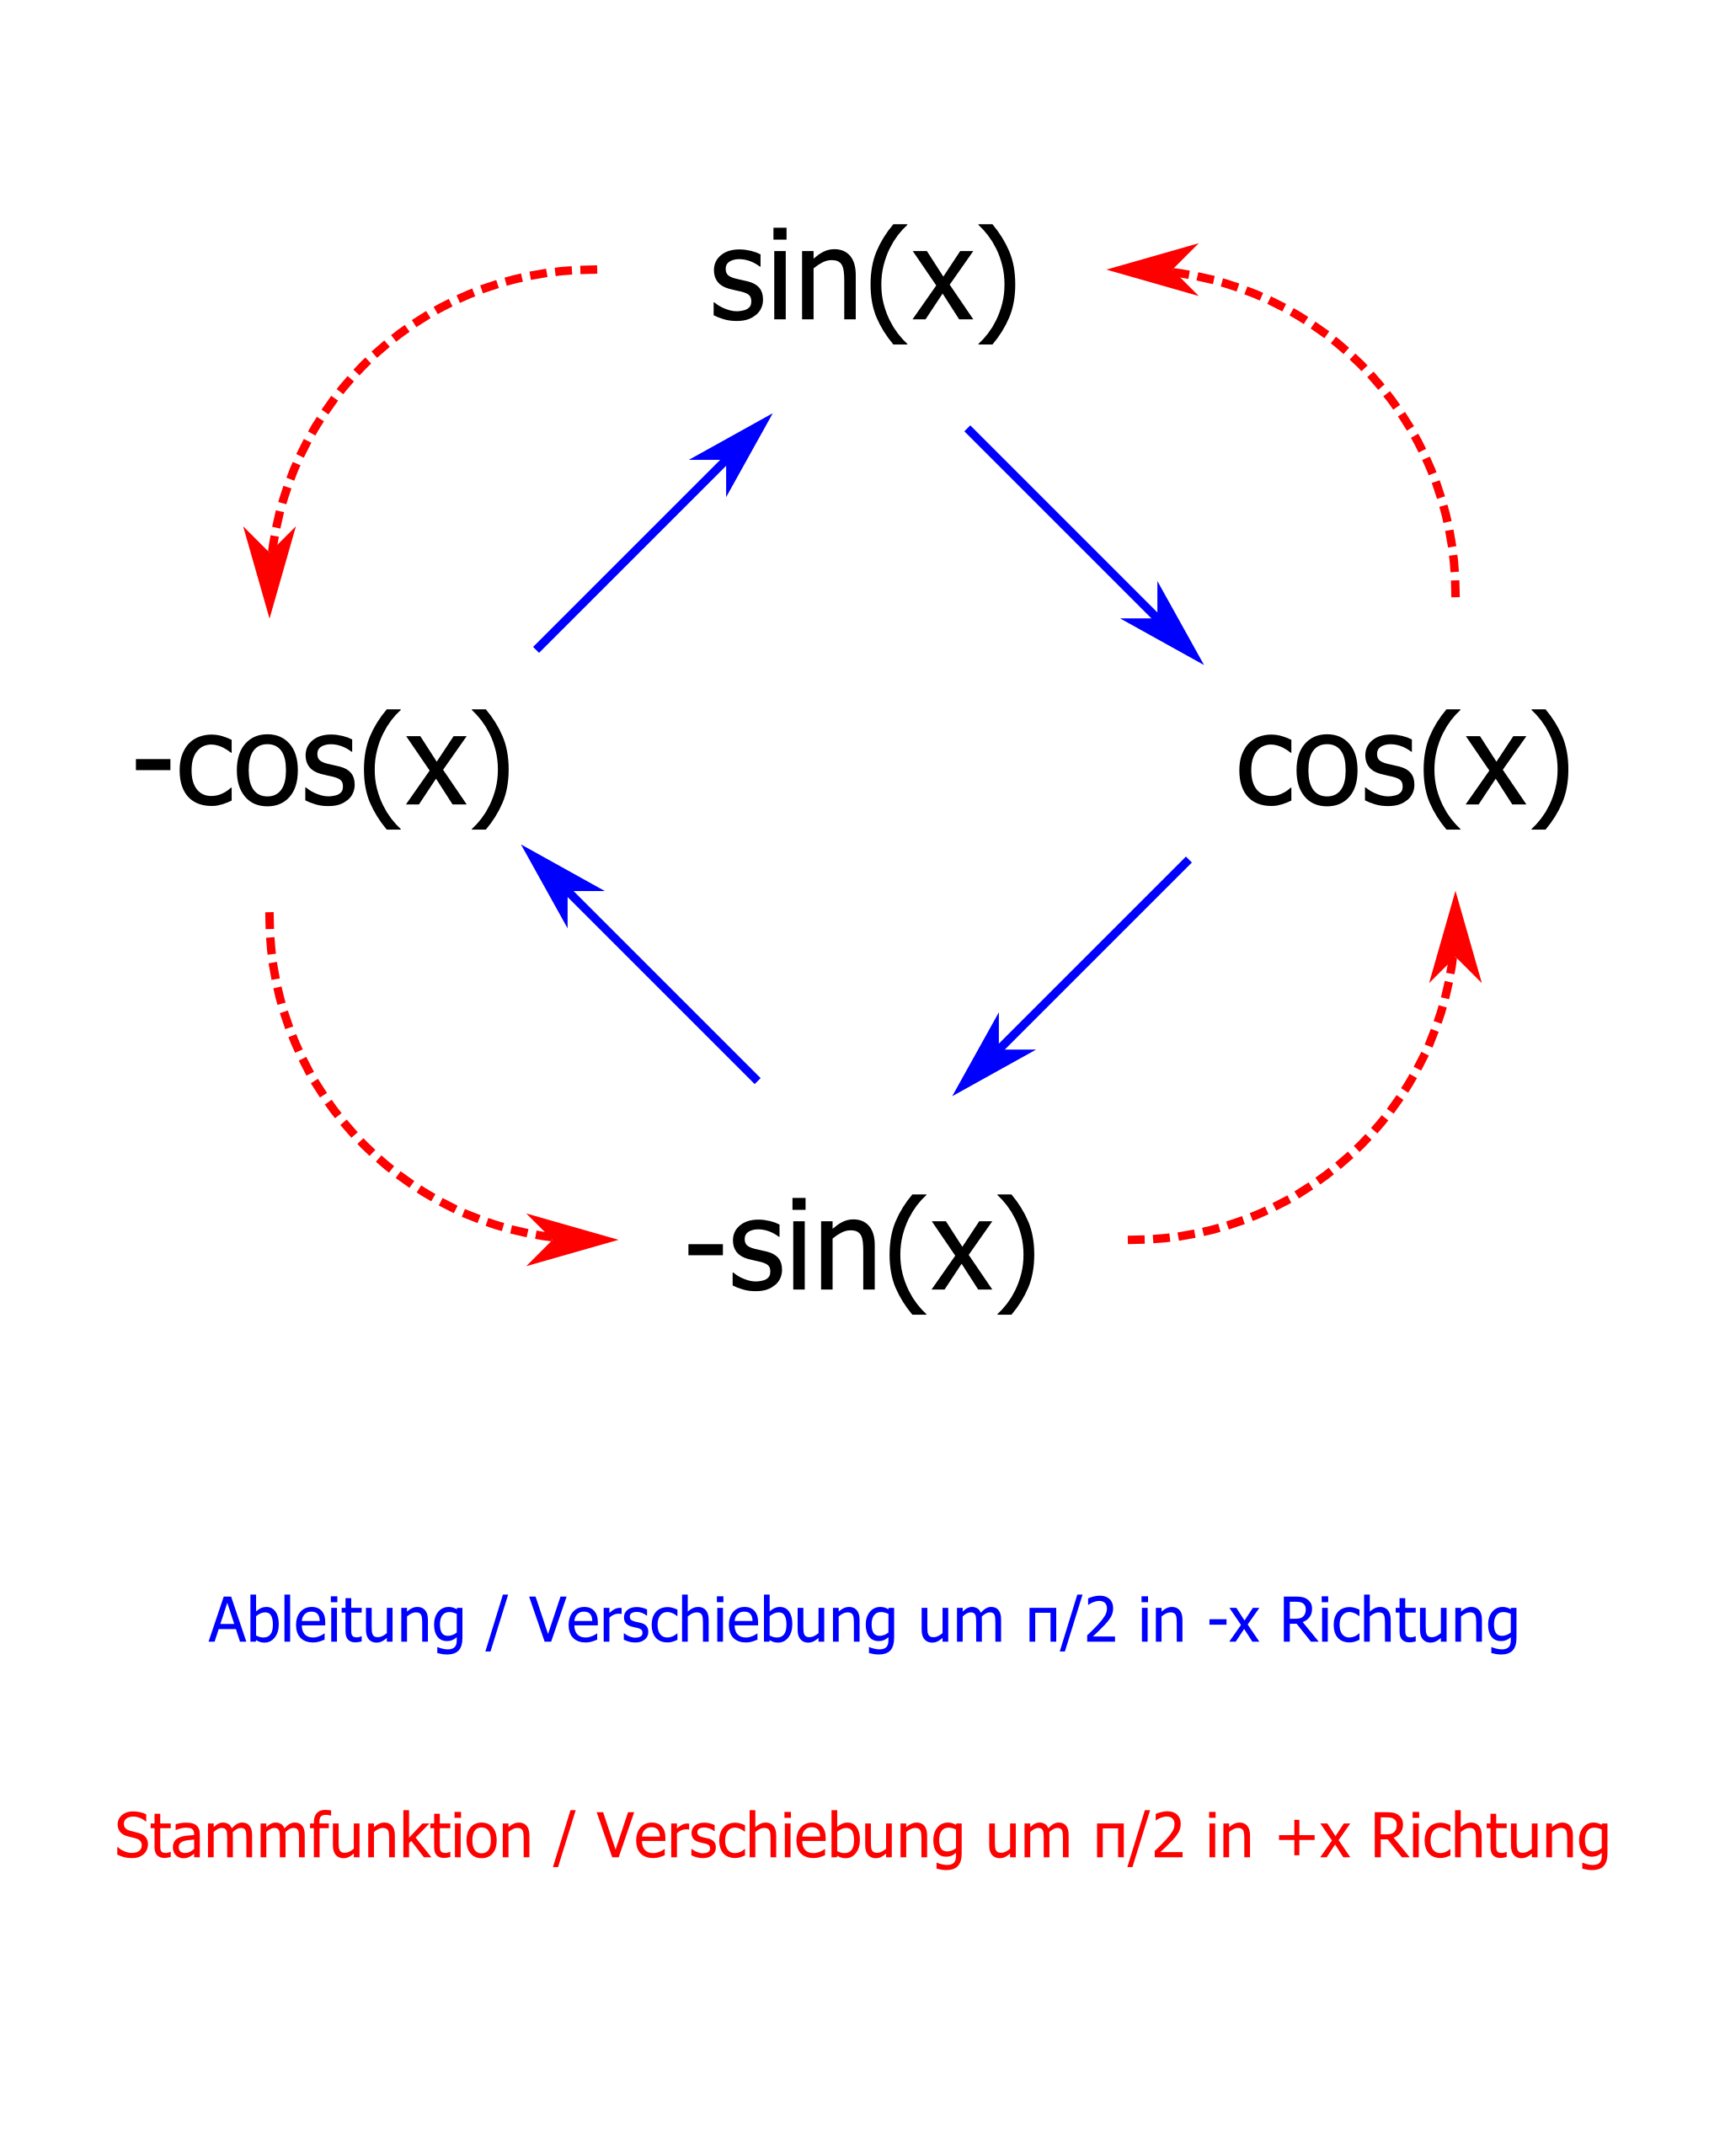
\includegraphics[width=0.45\linewidth]{Ableitungskreis.png}
    \captionsetup{labelformat=empty}
\end{figure}

\subsection*{Allgemeine Sinusfunktion}

$f\left(x\right)=a\cdot\sin\left(b\cdot\left(x+c\right)\right)+d$ \\

\noindent a: Änderung der Amplitude (Streckung oder Stauchung in y-Richtung) \\
b: Änderung der Periode (Steckung oder Stauchung in x-Richtung) \\
c: Verschiebung um c nach links (-x-Richtung) \\
d: Verschiebung um d nach oben (+y-Richtung)

\subsection*{Aufgaben}

\begin{enumerate}[label=$\alph*)$]
    \item $ \sin{(-90^\circ)} $
    \item $ \cos{(\theta + \frac{\pi}{2})} $ und $ \sin{(\theta - \frac{\pi}{2})} $
    \item $ \sin{(2\pi - 30°)} $
    \item Lösungsmenge für $ \sin{n \cdot 2\pi - 90°} $
    \item Beweise die ersten drei Eigenschaften mit Hilfe des Additionstheorems.
\end{enumerate}

\end{document}